\documentclass[a4paper]{article}
\usepackage[14pt]{extsizes} % для того чтобы задать нестандартный 14-ый размер шрифта
\usepackage[utf8]{inputenc}
\usepackage[russian]{babel}
\usepackage{setspace,amsmath}
\usepackage[left=20mm, top=15mm, right=15mm, bottom=15mm, nohead, footskip=10mm]{geometry} % настройки полей документа %последний язык является активным в документе
\usepackage{url}
\usepackage{graphicx}
\babelhyphenation[latin]{Mor-bi} %добавлен особый перенос

% for placeholder text
\usepackage{lipsum}


\begin{document}

% НАЧАЛО ТИТУЛЬНОГО ЛИСТА
\begin{center}
\hfill \break
\large{МИНЕСТЕРСТВО НАУКИ И ВЫСШЕГО ОБРОЗОВАНИЯ РОССИЙСКОЙ ФЕДЕРАЦИИ}\\
\footnotesize{ФЕДЕРАЛЬНОЕ ГОСУДАРСТВЕННОЕ АВТОНОМНОЕ ОБРАЗОВАТЕЛЬНОЕ УЧРЕЖДЕНИЕ}\\ 
\footnotesize{ВЫСШЕГО ПРОФЕССИОНАЛЬНОГО ОБРАЗОВАНИЯ}\\
\small{\textbf{УРАЛЬСКИЙ ФЕДЕРАЛЬНЫЙ УНИВЕРСИТЕТ}}\\
\small{\textbf{имени первого Президента России Б.Н.Ельцина}\\
\hfill \break
\normalsize{ИНСТИТУТ ЕСТЕСТВЕННЫХ НАУК И МАТЕМАТИКИ}\\
 \hfill \break
\normalsize{Кафедра прикладной математики и механики}\\
\hfill\break
\hfill \break
\hfill \break
\hfill \break
\large{РЕШЕНИЕ ЗАДАЧИ ПЕНЛЕВЕ-РАУСА}\\
\hfill \break
\hfill \break
\hfill \break
\normalsize{Магистерская диссертация\\
\hfill \break
Направление  01.04.03 "Механика и математическое моделирование"\\
\hfill \break
\hfill \break
\end{center}

\normalsize{ 
\begin{tabular}{lcc}
Зав.кафедрой & \hspace{1cm} & Магистерская диссертация\\
к. ф.-м. н., проф. А.\,Н. Сесекин& \hspace{1cm} &\\
& \hspace{1cm} &\\
\makebox[6cm]{\hruleffil} & \hspace{1cm} & {\bf Филимоновой}\\
& \hspace{1cm} & {\bf Марии Андреевны}\\
& \hspace{1cm} &\\
& \hspace{1cm} & \makebox[6cm]{\hruleffil} \\
& \hspace{1cm} &\\
Нормоконтролер: & \hspace{1cm} & Научный руководитель:\\
к. ф.-м. н., доц. \, & \hspace{1cm} А.\,Е.Шнейдер \\
& \hspace{1cm} &\\
\makebox[6cm]{\hruleffil} & \hspace{1cm} &
\makebox[6cm]{\hruleffil}\\
\end{tabular}
}\\
\hfill \break
\hfill \break
\begin{center} Екатеринбург 2019 \end{center}
\thispagestyle{empty} % выключаем отображение номера для этой страницы
 
% КОНЕЦ ТИТУЛЬНОГО ЛИСТА
 
\newpage
     
\tableofcontents % Вывод содержания
\newpage
 
\newpage
\section{Введение}{Введение} 
       В теоретической механике на практике часто встречаются задачи о движении ведущего и ведомого колес с сухим трением. Эта задача, которая встречается во многих практических случаях. 
       В данной работе будем исследовать плоское движение однородного шара при наличии трения. В этой задаче возникает много различных случаев: качение с проскальзыванием, качение без проскальзывания. Будем использовать методики решения задач Пенлеве с качением.


\newpage
\section{Трение Скольжения}{Трение Скольжения}  
При движении тела по поверхности в ходе соприкосновения возникает сила трения скольжения (Рис.1).
Все поверхности тел в той или иной степени шероховаты и все тела деформируемы. В связи с этим и сила реакции $\overline{R}$ шероховатой поверхности при равновесии тела зависит от активных сил не только по числовой величине, но и направлению. 

Если силу реакции $\overline{R}$ шероховатой поверхности разложить на составляющие, одна из которых $\overline{N}$ направлена по общей нормали к поверхности соприкосновения, а другая $\overline{F}$ находится в касательной плоскости к этой поверхности, то составляющая $\overline{F}$ силы реакции является силой трения скольжения, а составляющая $\overline{N}$ нормальной реакцией.

\begin{center}
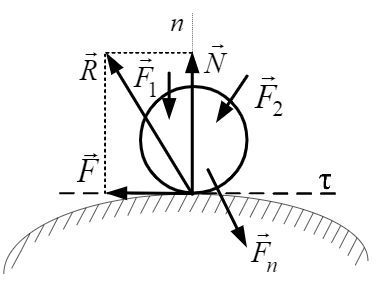
\includegraphics[scale=0.8]{1.png}\\
{\small Рис.1}
\end{center}

\newpage
\section{Постановка задачи Пенлеве-Рауса}{Постановка задачи Пенлеве-Рауса}
Однородный шар брошен без начальной угловой скорости прямолинейно вверх по шероховатой поверхности, наклоненной к горизонту под углом $\alpha$. Коэффициент трения f. Показать, что полное время, в течение которого шар поднимался по плоскости, будет таким же, как и в случае гладкой плоскости, и что время, в течение которого он скользил, относится по времени, в течение которого он катится как $\frac{2tg\alpha}{7f}$.

\subsection{Решение задачи Пенлеве-Рауса}
Пусть $\overline{v}$ - скорость центра шара,
\newline $\overline{\omega}$- его угловая скорость (скорость качения шара, т.к. задача плоская),
\newline m- масса шара,
 \newline r- радиус шара.
\subsection{Случай 1. Движение со скальжением}
 Имеем начальные условия из задачи Рауса:
 $$
 v(0)= v_0;
 $$
$$
\omega (0)= \omega_0.
$$
Обозначим $v_1=v-r\omega$ – скорость точки касания шара. В этой точке возникает сила трения F, удовлетворяющая условиям:

$$
\overline{F} =- \frac{\bar{v_1}}{|\bar{v_1}|} fmg \cdot cos \alpha ;   v_1 \neq 0, 
$$


$$
|\overline{F}|\leq fmg \cdot cos \alpha; v_1=0.
$$


\newline Уравнение движения при $ v_1 ≠ 0 : 


$$
m \dot{\omega} = - mg \cdot sin \alpha - fg \cdot cos \alpha \cdot (sign v_1)
$$


$$
\frac{2}{5} mr^2 \dot{\omega} = fmg \cdot cos \alpha \cdot (sign v_1) \cdot r .
$$

Так как $f \geq \frac{2}{7} tg \alpha ,$ то $v_1(t)$ монотонно убывает от $v_1(0)$ до нуля по закону:
$$
\dot{v_1}(0) = - g sin \alpha - \frac{2}{7} fg cos \alpha . \eqno(1) 
$$
\newlineПроинтегрируем уравнение (1),чтобы найти время подъема со сольжением. Получаем:
$$
t_1 = {v_0 \over{g sin \alpha + {7 \over{2}} fg cos \alpha}}.
$$


\begin{thebibliography}{7}
\bibitem{Rozenblat} Розенблат~Г.~М. Динамические системы с сухим трением. -Москва-Ижевск: НИЦ «Регулярная и хаотическая динамика», 2006.
\bibitem{Rauth} Раус ~Э. Динамика системы тверды тел: Пер. с англ. В 2-х томах. Т. I/Под ред. ~Ю.~А. Архангельского и ~В.~Г. Дёмина. – М.: Наука. Главная редакция физико-математической литературы, 1983.
\bibitem{Penleve} ~П. Пэнлеве. Лекции о трении. Под ред. ~Д.~В. Жарков. 1954 г.
\bibitem{Rauth} Раус ~Э. Динамика системы тверды тел: Пер. с англ. В 2-х томах. Т. II/Под ред. ~Ю.~А. Архангельского и ~В.~Г. Дёмина. – М.: Наука. Главная редакция физико-математической литературы, 1983.
\end{thebibliography}

\end{document}

